% A simple template for Beamer presentations in LaTeX
% 
% To produce pdf run:
%   $ pdflatex beamer.tex 
%

\documentclass{beamer}
\usetheme{Singapore}

\AtBeginSection[]
{
  \begin{frame}
    \frametitle{Outline}
    \tableofcontents[currentsection]
  \end{frame}
}

\hypersetup{colorlinks=true}

% Graphics examples
%\centerline{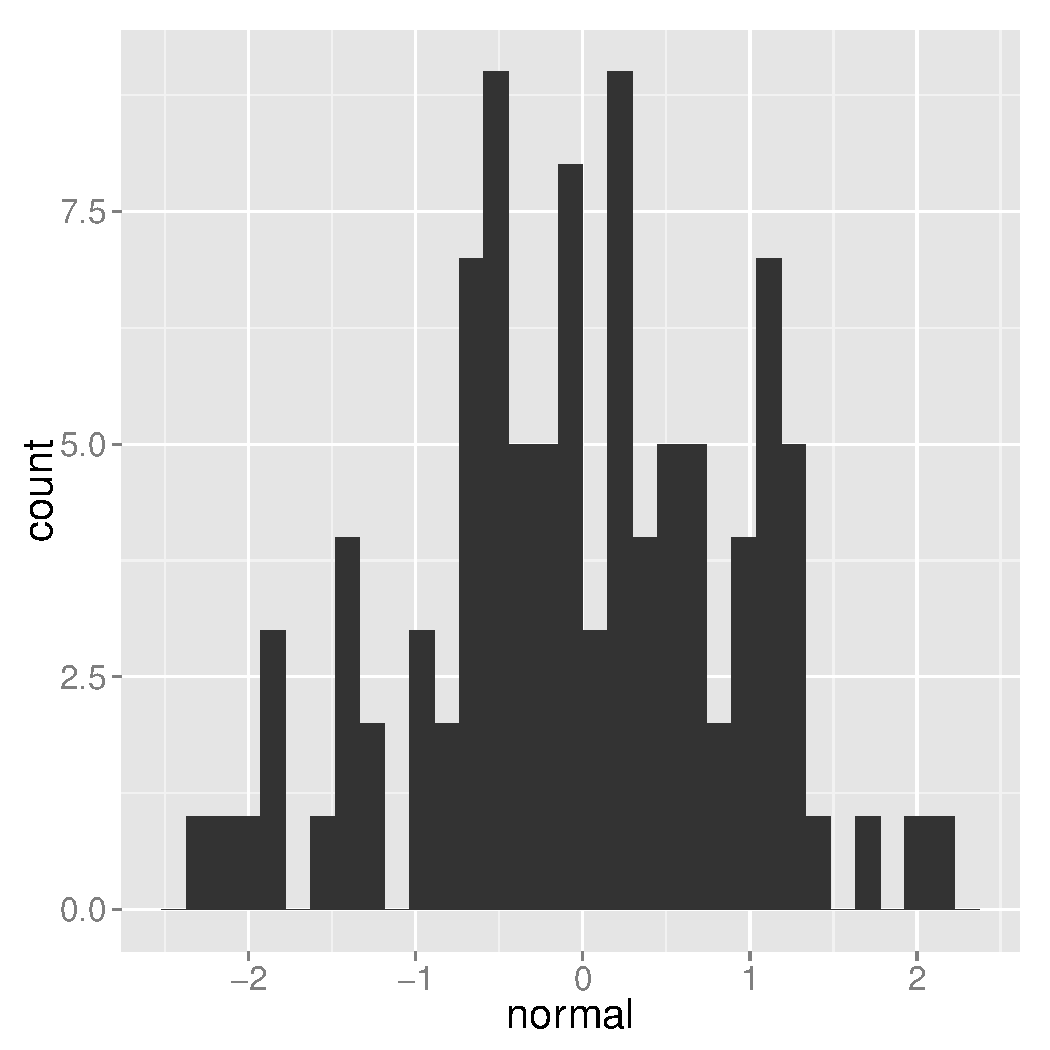
\includegraphics[height=2.5in]{figs/normal.pdf}}
%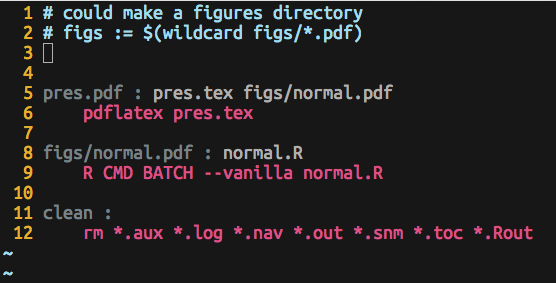
\includegraphics[width=4in]{figs/makefile.png}

%%%%%%%%%%%%%%%%%%%%%%%%%%%%%%%%%%%%%%%%%%%%%%%%%%%%%%%%%%%%

\begin{document}

\title{Data Revolution}
\subtitle{A journey from Red Bluff to Big Data}
\author{Clark Fitzgerald - @clarkfitzg}
\institute{Red Bluff High School}
\date{21 August 2014}

\frame{\titlepage}


%%%%%%%%%%%%%%%%%%%%%%%%%%%%%%%%%%%%%%%%%%%%%%%%%%%%%%%%%%%%
\begin{frame}


\frametitle{Goals Today}

\begin{itemize}
\item What I wish I would've known...
\item A sense of possibility around math and data
\end{itemize}

\tableofcontents


\end{frame}
%%%%%%%%%%%%%%%%%%%%%%%%%%%%%%%%%%%%%%%%%%%%%%%%%%%%%%%%%%%%
\section{Personal Journey}
%%%%%%%%%%%%%%%%%%%%%%%%%%%%%%%%%%%%%%%%%%%%%%%%%%%%%%%%%%%%
\begin{frame}


\frametitle{The Army }

\centerline{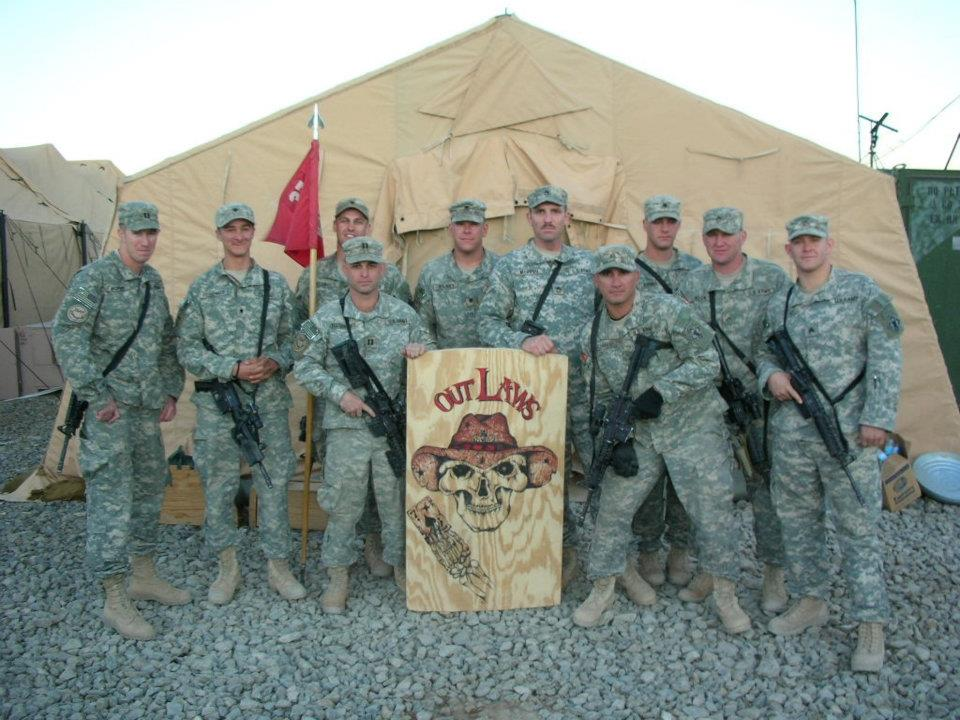
\includegraphics[height=2.5in]{figs/army.jpg}}


\end{frame}
%%%%%%%%%%%%%%%%%%%%%%%%%%%%%%%%%%%%%%%%%%%%%%%%%%%%%%%%%%%%
\begin{frame}


\frametitle{Mountain Guide }

\centerline{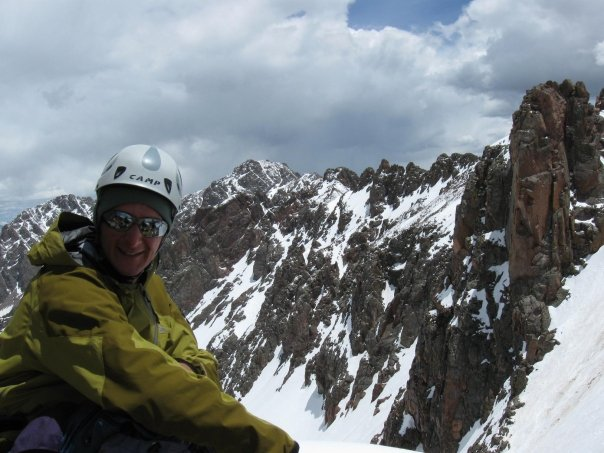
\includegraphics[height=2.5in]{figs/mountains.jpg}}


\end{frame}
%%%%%%%%%%%%%%%%%%%%%%%%%%%%%%%%%%%%%%%%%%%%%%%%%%%%%%%%%%%%
\begin{frame}


\frametitle{Marriage to Yeji}

\centerline{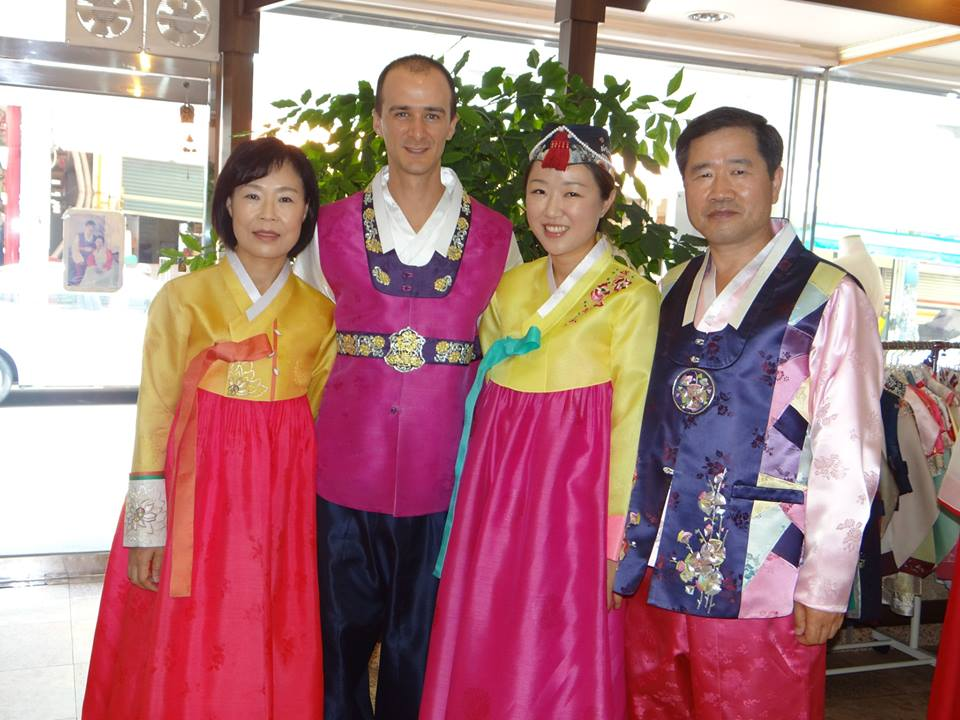
\includegraphics[height=2.5in]{figs/korea.jpg}}


\end{frame}
%%%%%%%%%%%%%%%%%%%%%%%%%%%%%%%%%%%%%%%%%%%%%%%%%%%%%%%%%%%%
\begin{frame}


\frametitle{Math at Shasta then UC Berkeley }

\centerline{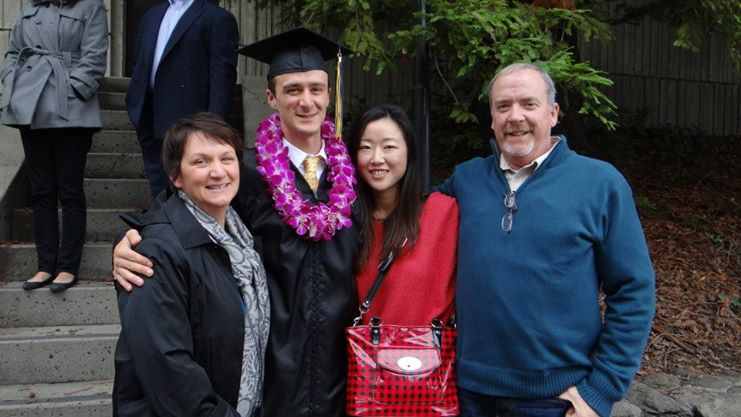
\includegraphics[height=2.5in]{figs/berkeley.jpg}}


\end{frame}
%%%%%%%%%%%%%%%%%%%%%%%%%%%%%%%%%%%%%%%%%%%%%%%%%%%%%%%%%%%%
\begin{frame}


\frametitle{Cisco Systems}

\centerline{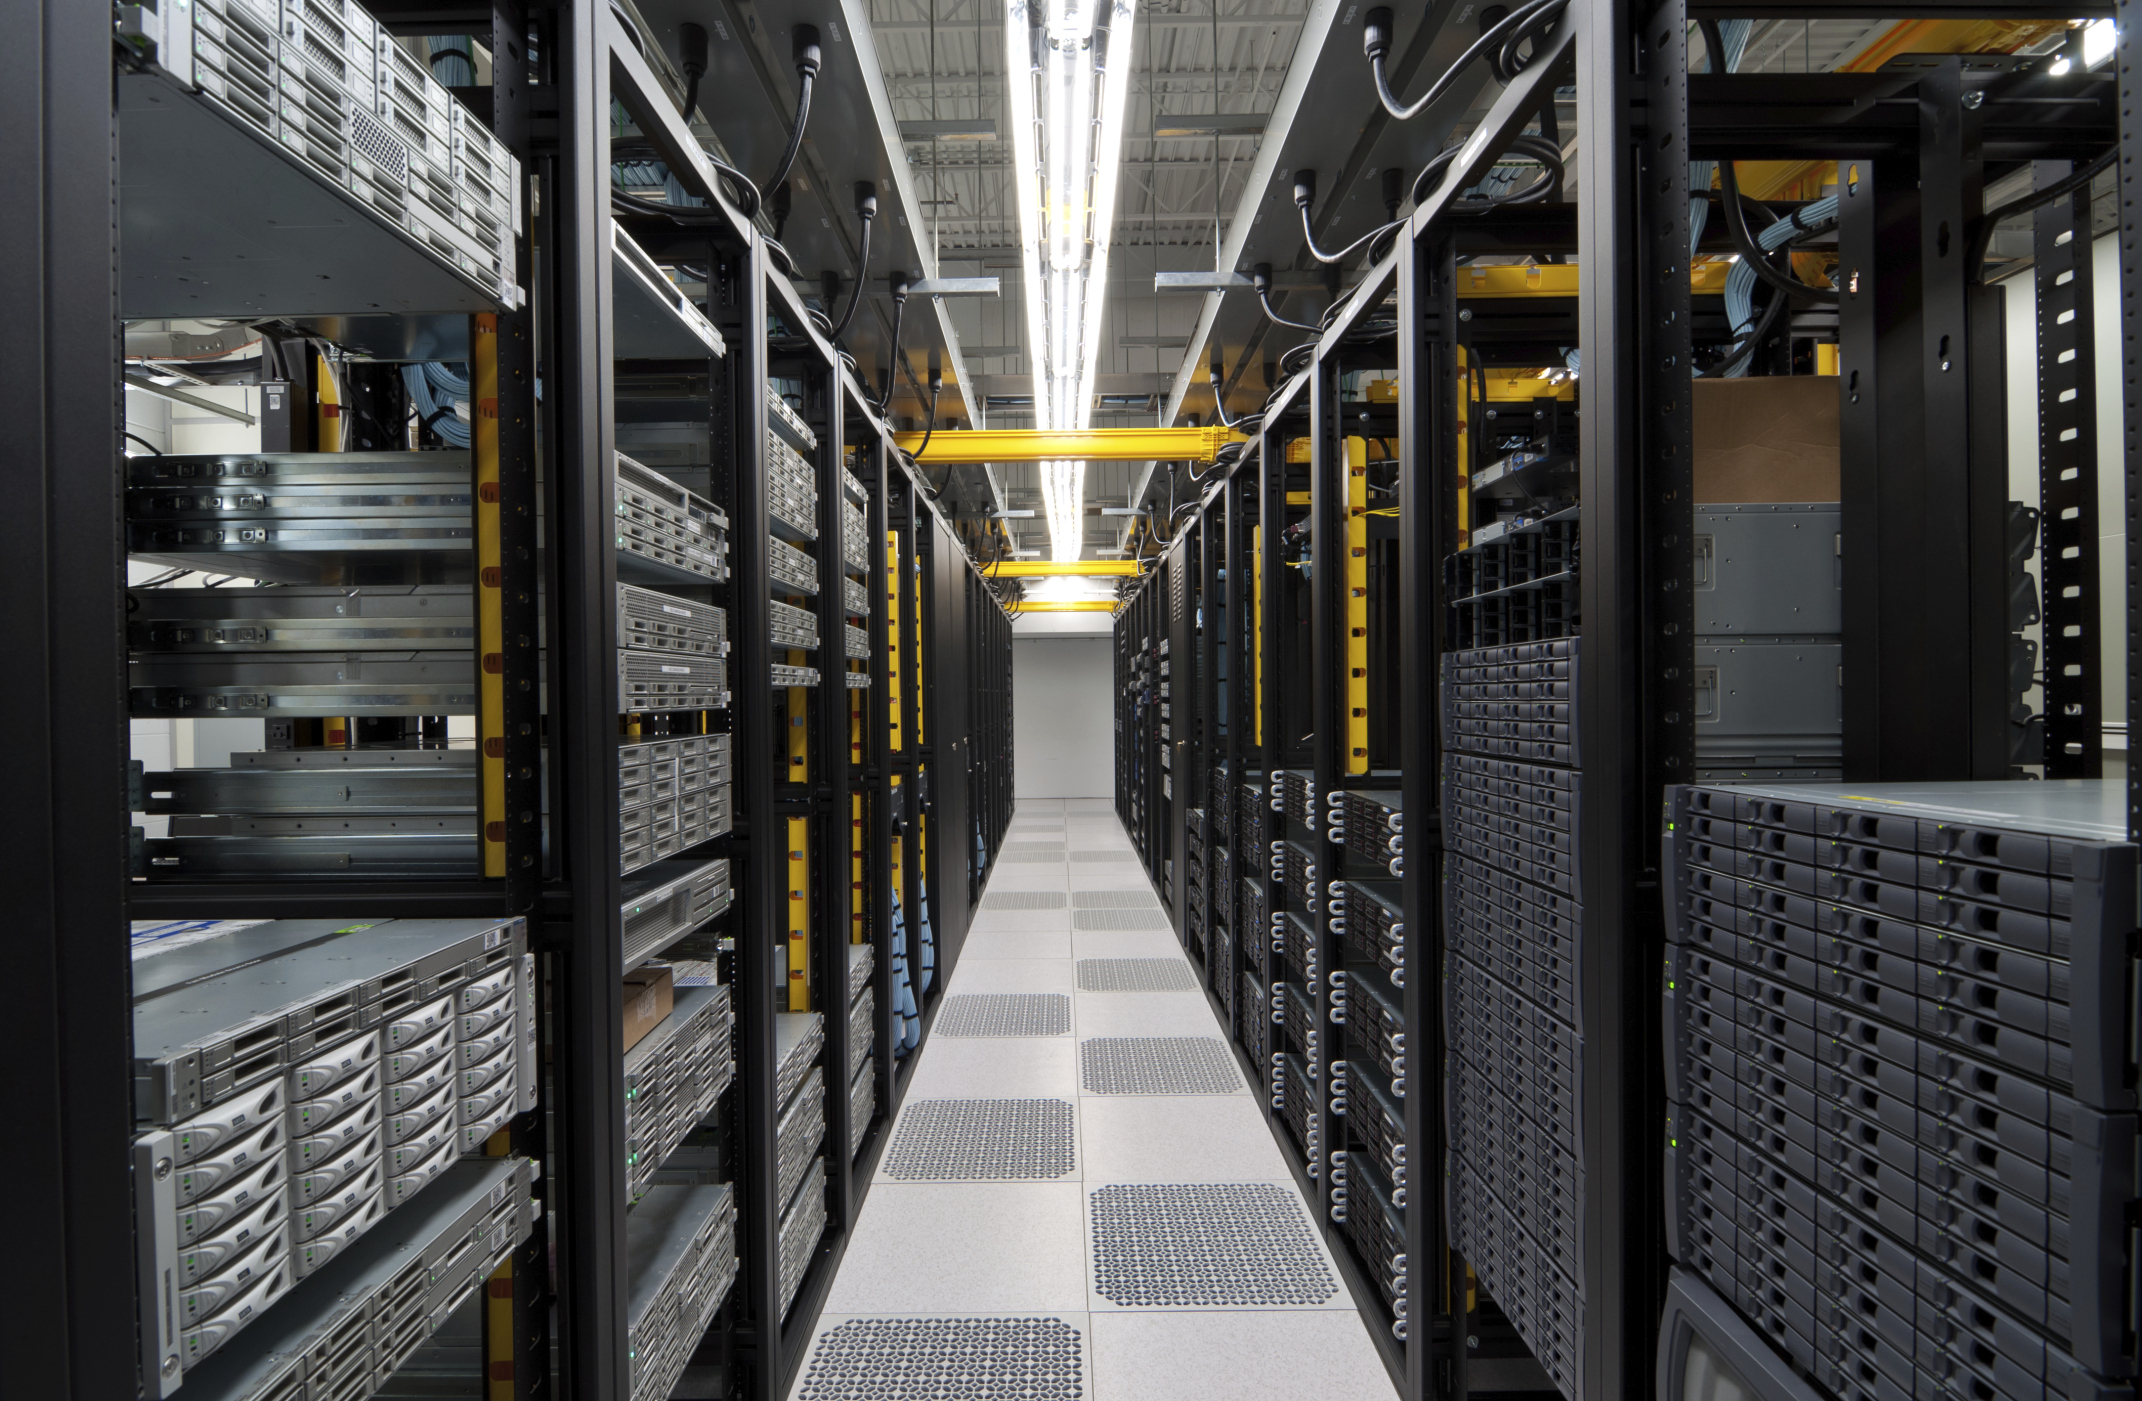
\includegraphics[height=2.5in]{figs/datacenter.jpg}}


\end{frame}
%%%%%%%%%%%%%%%%%%%%%%%%%%%%%%%%%%%%%%%%%%%%%%%%%%%%%%%%%%%%
\begin{frame}


\frametitle{UC Davis - Phd in Statistics}

\centerline{
\includegraphics[width=4in]{figs/davis.png}}


\end{frame}
%%%%%%%%%%%%%%%%%%%%%%%%%%%%%%%%%%%%%%%%%%%%%%%%%%%%%%%%%%%%
\section{Big Data}
%%%%%%%%%%%%%%%%%%%%%%%%%%%%%%%%%%%%%%%%%%%%%%%%%%%%%%%%%%%%
\begin{frame}

\frametitle{What is Data?}

Data is information.

\begin{itemize}
\item Facebook friends
\item Amazon product pricing
\item bank account balance
\item text messages
\item traffic sensors
\item daily sales at WalMart
\item words in a book
\item pixels in an image
\end{itemize}


\end{frame}
%%%%%%%%%%%%%%%%%%%%%%%%%%%%%%%%%%%%%%%%%%%%%%%%%%%%%%%%%%%%
\begin{frame}[fragile]


\frametitle{An example of data}

Pixels in an image, transformed into a table:

\begin{verbatim}
$ head python_logo.csv
x,y,blue,green,red
0,0,255,255,255
1,0,255,255,255
2,0,255,255,255
3,0,255,255,255
4,0,255,255,255
5,0,255,255,255
6,0,255,255,255
7,0,255,255,255
8,0,255,255,255
\end{verbatim}


\end{frame}
%%%%%%%%%%%%%%%%%%%%%%%%%%%%%%%%%%%%%%%%%%%%%%%%%%%%%%%%%%%%
\begin{frame}


\frametitle{Normal Data}

10,000 normally distributed points

\centerline{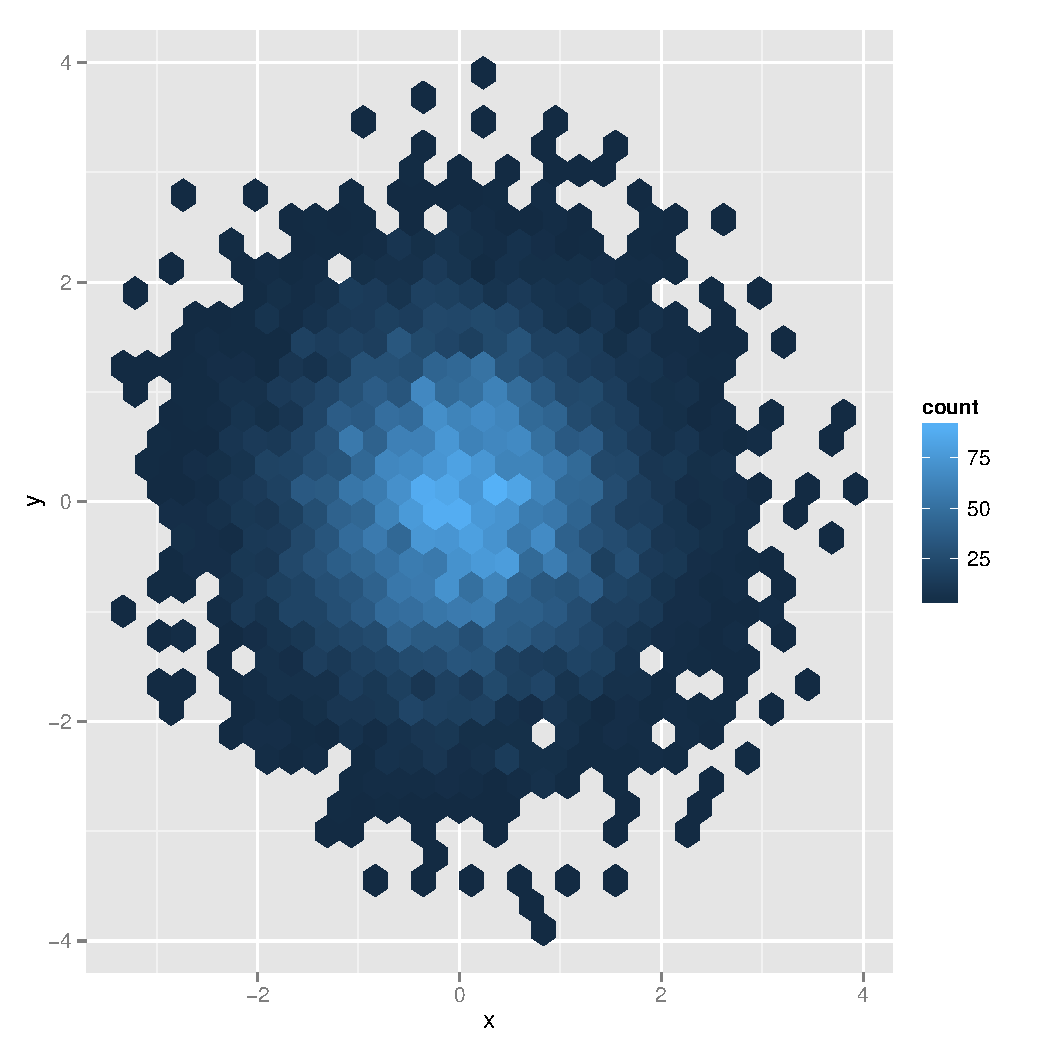
\includegraphics[height=3in]{normal.pdf}}


\end{frame}
%%%%%%%%%%%%%%%%%%%%%%%%%%%%%%%%%%%%%%%%%%%%%%%%%%%%%%%%%%%%
\section{Opportunity}
%%%%%%%%%%%%%%%%%%%%%%%%%%%%%%%%%%%%%%%%%%%%%%%%%%%%%%%%%%%%
\begin{frame}


\frametitle{It's like the Gold Rush!}
\centerline{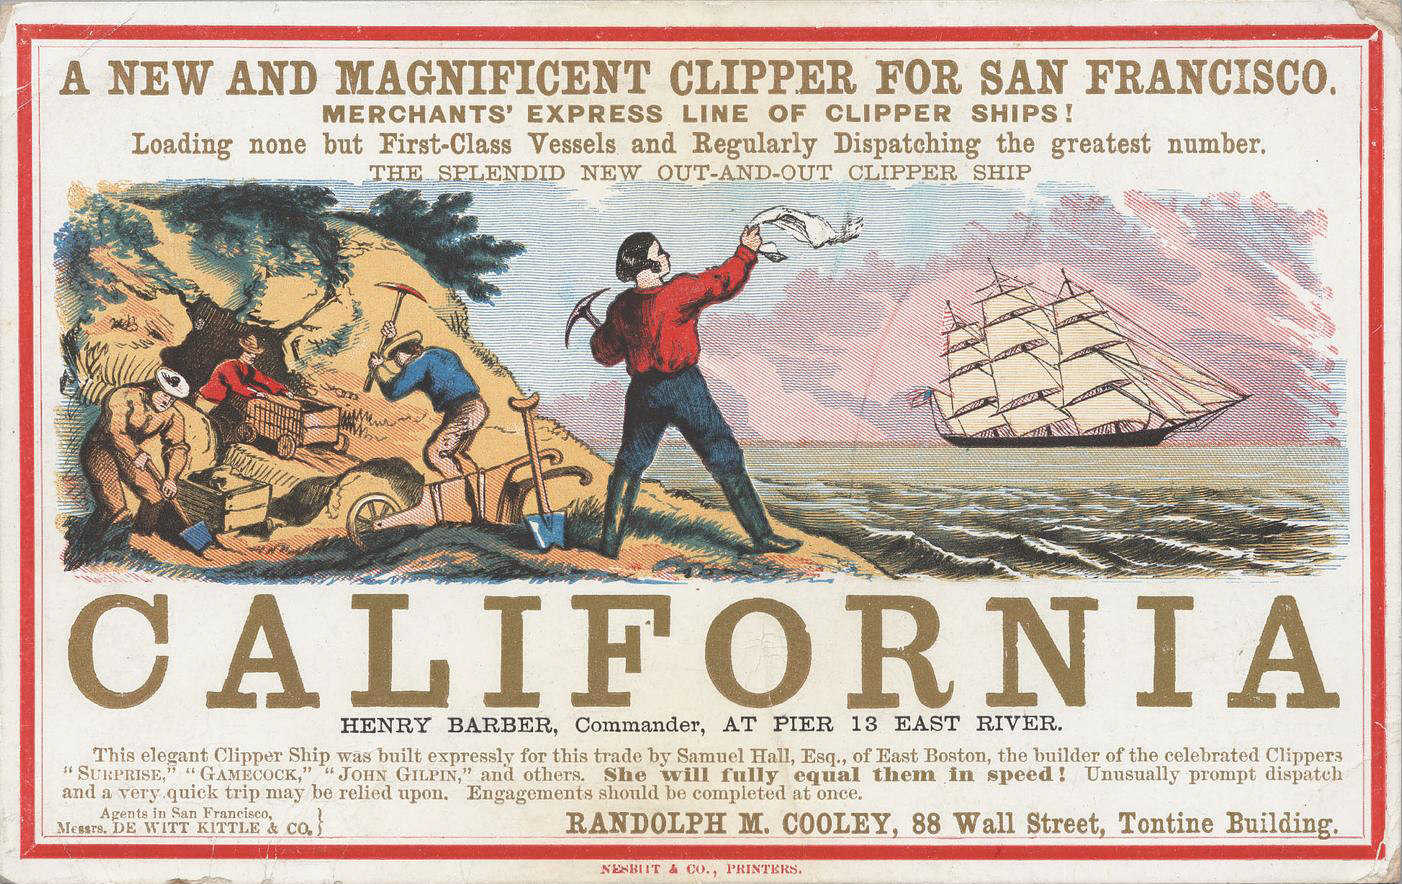
\includegraphics[height=2.5in]{figs/goldrush.jpg}}


\end{frame}
%%%%%%%%%%%%%%%%%%%%%%%%%%%%%%%%%%%%%%%%%%%%%%%%%%%%%%%%%%%%
\begin{frame}


Why is it like the Gold Rush?


\end{frame}
%%%%%%%%%%%%%%%%%%%%%%%%%%%%%%%%%%%%%%%%%%%%%%%%%%%%%%%%%%%%
\begin{frame}


Because few have the skills.

\begin{itemize}
\item \Huge{Statistics}
\item \Huge{Programming}
\item \Huge{Mathematics}
\end{itemize}

\end{frame}
%%%%%%%%%%%%%%%%%%%%%%%%%%%%%%%%%%%%%%%%%%%%%%%%%%%%%%%%%%%%
\begin{frame}[fragile]


\frametitle{Code to process a large data set}

\begin{verbatim}

import csv
import collections

count = collections.Counter()

with open('Train.csv') as Train:
    for row in csv.DictReader(Train):
        # split tag column on spaces
        tags = row['Tags'].split(' ')
        count.update(tags)

\end{verbatim}


\end{frame}
%%%%%%%%%%%%%%%%%%%%%%%%%%%%%%%%%%%%%%%%%%%%%%%%%%%%%%%%%%%%
\begin{frame}


You can start learning this stuff \emph{today!}

Everything is free and open access.

\begin{figure}
   
\includegraphics[width=0.4\textwidth]{figs/coursera.png}
   \hfill
   
\includegraphics[width=0.4\textwidth]{figs/r.png}
\end{figure}

\centerline{
\includegraphics[height=1in]{figs/python.jpeg}}

\end{frame}
%%%%%%%%%%%%%%%%%%%%%%%%%%%%%%%%%%%%%%%%%%%%%%%%%%%%%%%%%%%%
\section{Wrapping up}
%%%%%%%%%%%%%%%%%%%%%%%%%%%%%%%%%%%%%%%%%%%%%%%%%%%%%%%%%%%%
\begin{frame}


\frametitle{Goals Today Revisited}

\begin{itemize}
\item There is so much to do!

Find something you like.

\item This will help you in nearly \emph{any} field.
\end{itemize}


\end{frame}
%%%%%%%%%%%%%%%%%%%%%%%%%%%%%%%%%%%%%%%%%%%%%%%%%%%%%%%%%%%%
\begin{frame}


\huge{Questions?}


\end{frame}
%%%%%%%%%%%%%%%%%%%%%%%%%%%%%%%%%%%%%%%%%%%%%%%%%%%%%%%%%%%%

\end{document}
